\chapter{Results}
\label{cha:results}
In the following sections, the data from the dose of vibrationally excited molecules are presented. It was desireable to determine the threshold temperature of the hydrogenation of graphene, and hence the temperature of the doser was changed in order to shift the distribution of vibrationally excited states. Therefore the data includes dosages at temperatures of, 1343\degree C, 1543\degree C and 1745\degree C. A dose at 1300\degree C were performed as well, however the STM broke, and no pictures are therefore included.

\section{Graphene on Ir}

The quality of the graphene was checked each time D$_2$ was dosed on the sample, in order to ensure that the amount of defects was at a minimum. STM pictures of pure graphene on Ir(111) is shown in this section. On figure \ref{GrIr} pictures of graphene on Ir in different sizes is shown. Figure \ref{GrIr1} shows a large image of a graphene monolayer covering the Ir surface. Although the quality of the image is of low quality, the moire pattern is perceived. Also several step edges from the underlying Ir surface is seen. Several line scans has been performed on these edges, which show that the height difference is 2Å $\pm$0.4Å. This value is consistent with the value of 0.22nm found in the litterature.\cite{1367-2630-11-2-023006}\\
On figure \ref{GrIr2} a high resolution image of Gr/Ir is seen. The moire pattern is very prominent in this figure, and the spacing between the individual sites in the moire unit cell can be determined from a line scan. A line scan was drawn on figure \ref{GrIr2} and two points were positioned in the corners of the moire unit cell in order to obtain the moire periodicity. The morié periodicity is 25.2 $\pm$ 0.4Å according to the litterature.\cite{1367-2630-10-4-043033} This agrees with the measured length of 25.24 Å from the line scan. Typical defects on of the graphene monolayer is seen as well in this figure. Also the hexagonal pattern of graphene is sensed because of the atomic resolution. On figure \ref{GrIr3} the individual carbon atoms are even more clear.\\

\begin{figure}[H]
\makebox[\textwidth][c]{
  \begin{subfigure}[b]{0.3\paperwidth}
    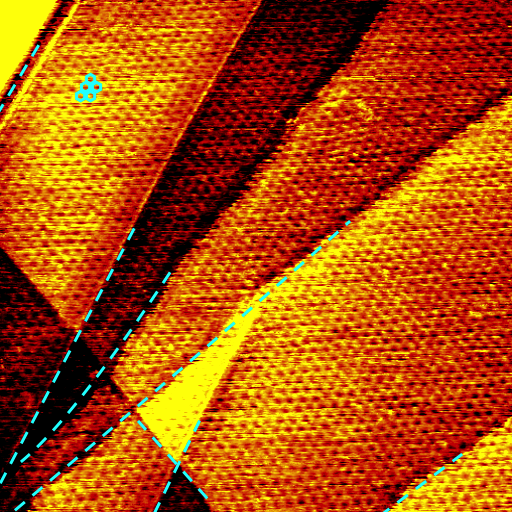
\includegraphics[height=\textwidth]{STMdata/FFT/2016-04-11_000_33.png}
    \caption{993x993 Å - 0.690 nA 78.1 mV}
    \label{GrIr1}
  \end{subfigure}
  \begin{subfigure}[b]{0.3\paperwidth}
    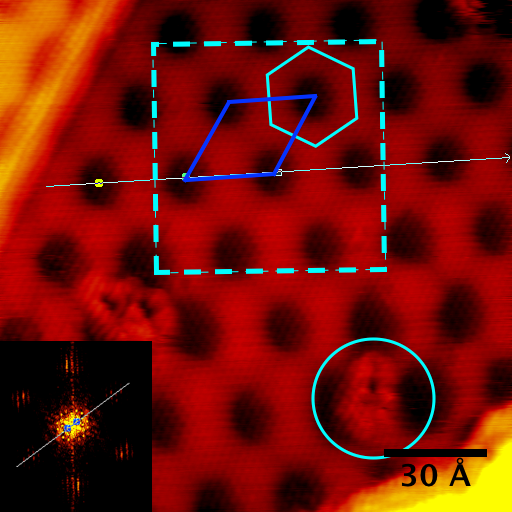
\includegraphics[height=\textwidth]{STMdata/FFT/2016-04-11_000_50.png}
    \caption{148x148 Å - -0.890 nA -311.3 mV}
    \label{GrIr2}
  \end{subfigure}
  \begin{subfigure}[b]{0.3\paperwidth}
    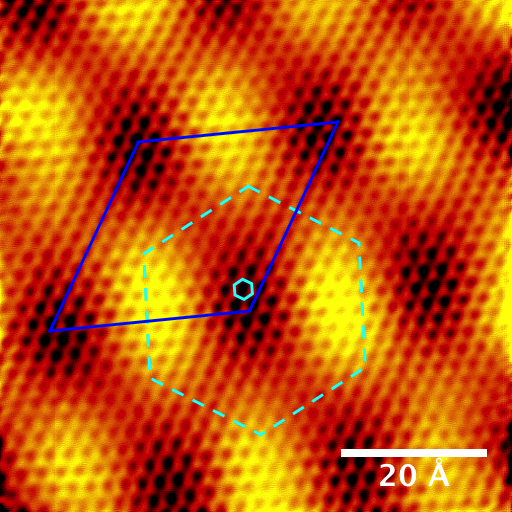
\includegraphics[height=\textwidth]{STMdata/FFT/2016-04-11_000_56.png}
    \caption{70x70 Å - 0.910 nA 311.3 mV}
    \label{GrIr3}
  \end{subfigure}
}
\caption{}
\label{GrIr}
\end{figure}

\section{D2 on graphene}

\subsection{Full hydrogen coverage}
In order to compare the results from dosing molecular hydrogen STM pictures were taken of a fully hydrogenated surface. On figure \ref{D2:full} images of different scales can be seen. The surface was hydrogenated by filling the chamber with hydrogen at a pressure of $1.02 \cdot 10^{-5}$mbar and leaving the ion gauge on for 12 hours. As seen on figure \ref{full:1} the sample is not just locally hydrogenated. A line scan was performed on the sample in order to check the periodicity of the hydrogenation. The line scan is seen on figure \ref{full:3} and the distance between the two points is measured to 24.2Å. This value is very close to the periodicity of the moiré unit cell, which is expected.\\
As seen on figure \ref{full:2}, the most common pattern, of the hydrogenated surface, is ring shaped structures with a bright rim and a darker center. By comparing figure \ref{full:2} with figure \ref{GrIr2} it is obvious that the adsorption of hydrogen on the surface changes the LDOS. It is noticeable that the defects on figure \ref{GrIr2} looks like the ring shaped structures seen on figure \ref{D2:full}, and hence these defect might be the caused by adsorbed hydrogen. Furthermore some areas of the saturated surface seem to melt together in a bigger structure, seen as the bone- and three point star shaped structures on figure \ref{full:2}.

\begin{figure}[H]
\makebox[\textwidth][c]{
  \begin{subfigure}[b]{0.3\paperwidth}
    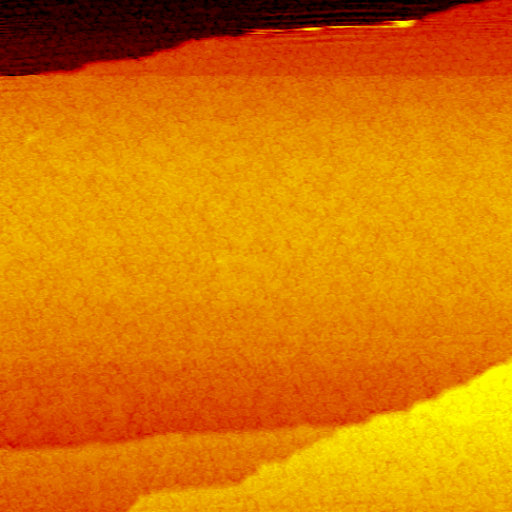
\includegraphics[height=\textwidth]{STMdata/FFT/2016-04-13_001_15.png}
    \caption{949x949 Å - 0.860 nA 67.1 mV}
    \label{full:1}
  \end{subfigure}
  \begin{subfigure}[b]{0.3\paperwidth}
    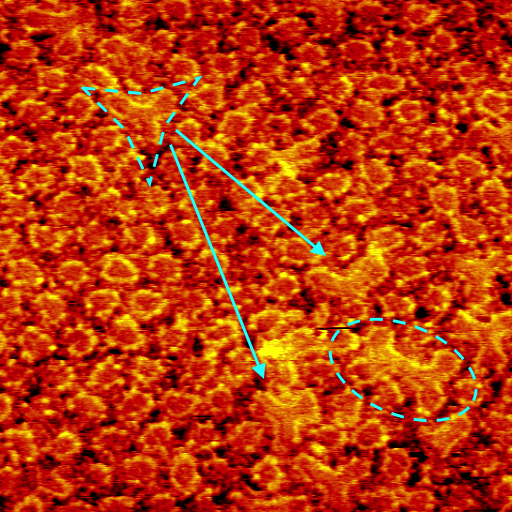
\includegraphics[height=\textwidth]{STMdata/FFT/2016-04-13_001_4.png}
    \caption{497x497 Å - 0.850 nA 73.5 mV}
    \label{full:2}
  \end{subfigure}
  \begin{subfigure}[b]{0.3\paperwidth}
    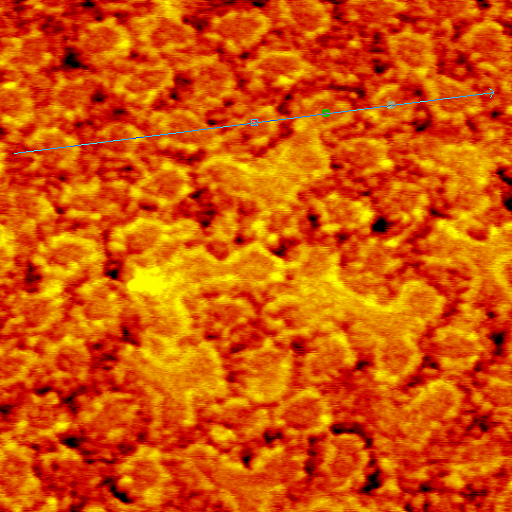
\includegraphics[height=\textwidth]{STMdata/FFT/2016-04-13_001_13.png}
    \caption{150x150 Å - 0.850 nA 73.5 mV}
    \label{full:3}
  \end{subfigure}
}
\caption{Fully hydrogenated Gr/Ir surface.}
\label{D2:full}
\end{figure}


\subsection{1745\degree C dose}

This dose happened at a pirani pressure of $6.8 \cdot 10^{-2}$mbar, and with the doser at a temperature of 1745\degree C. The doseage time was 20 min. The graphene was checked before the dose in order to ensure that no abnormal amount of defects was present. Three images at different scales are shown in figure \ref{D2:1745}. These pictures were taken right after the dose had ended, and the pressure dropped sufficiently. As seen on figure \ref{D2:17451}, the surface is far from saturated, compared to figure \ref{full:1}. It is also worth noting that none of the hydrogenated sites melt together to form bigger structures, which indicates that this phenomenon happens after the surface has been saturated.\\
Individual hydrogen atoms are not distinguishable from the STM images, and therefore the coverage is estimated as a percentage of the number of hydrogenated sites, compared to the total number of unit cells. Figures \ref{D2:17452} and \ref{D2:17453} were used to calculate an estimate of the saturation of the surface. The coverage on figure \ref{D2:17452} was calculated to 41\% and the coverage on figure \ref{D2:17453} was calculated to 29\%. This means that about one third of the surface is covered with hydrogen after a dosage of excited molecules for 20 min, at a chamber pressure of $5 \cdot 10^{-5}$mbar.

\begin{figure}[H]
\makebox[\textwidth][c]{
  \begin{subfigure}[b]{0.3\paperwidth}
    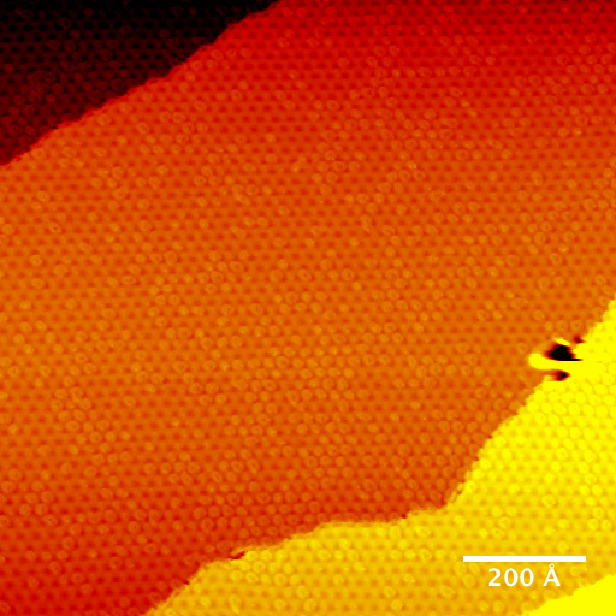
\includegraphics[height=\textwidth]{STMdata/FFT/2016-04-11_003_14.png}
    \caption{998x998 Å - 1.060 nA 67.1 mV}
    \label{D2:17451}
  \end{subfigure}
  \begin{subfigure}[b]{0.3\paperwidth}
    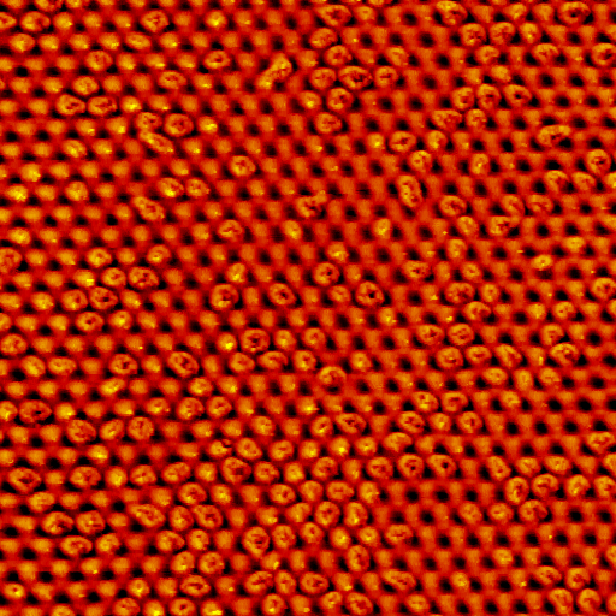
\includegraphics[height=\textwidth]{STMdata/FFT/2016-04-11_003_15.png}
    \caption{497x497 Å - 1.080 nA 67.1 mV}
    \label{D2:17452}
  \end{subfigure}
  \begin{subfigure}[b]{0.3\paperwidth}
    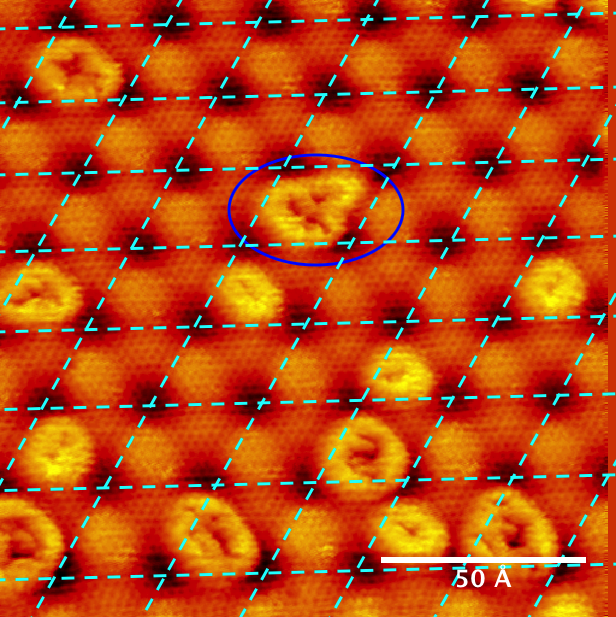
\includegraphics[height=\textwidth]{STMdata/FFT/2016-04-11_003_23.png}
    \caption{150x150 Å - 1.090 nA 67.1 mV}
    \label{D2:17453}
  \end{subfigure}
}
\caption{Hydrogenated Gr/Ir surface after dose of H$_2$ at a doser temperature of 1745\degree C.}
\label{D2:1745}
\end{figure}

\subsection{1593\degree C dose}

This dose happened at a pirani pressure of $6.8 \cdot 10^{-2}$mbar and a doser temperature of 1593\degree C. Again the dose had a duration of 20 min. The pictures from this dose are shown in figure \ref{D2:1593}. The resemblance between the pictures shown in figure \ref{D2:1745} and \ref{D2:1593} is quite high. Again the ring shaped structures are seen, and the shape of these are very similar to the ones observed earlier. Figures \ref{D2:15931} and \ref{D2:15932} were used to calculate the coverage of hydrogenation, with values of 32\% and 25\% respectively. These values are however very position dependant, and therefore they do not necessarily reflect the accurate coverage. It is however pretty obvious that some hydrogen has adsorbed to the surface.

\begin{figure}[H]
\makebox[\textwidth][c]{
  \begin{subfigure}[b]{0.3\paperwidth}
    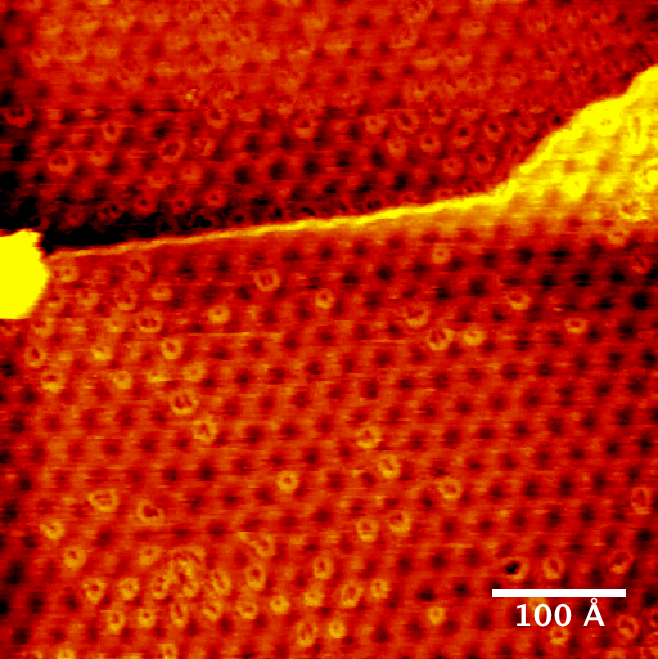
\includegraphics[height=\textwidth]{STMdata/FFT/2016-04-14_000_44.png}
    \caption{488x488 Å - 0.900 nA 190.4 mV}
    \label{D2:15931}
  \end{subfigure}
  \begin{subfigure}[b]{0.3\paperwidth}
    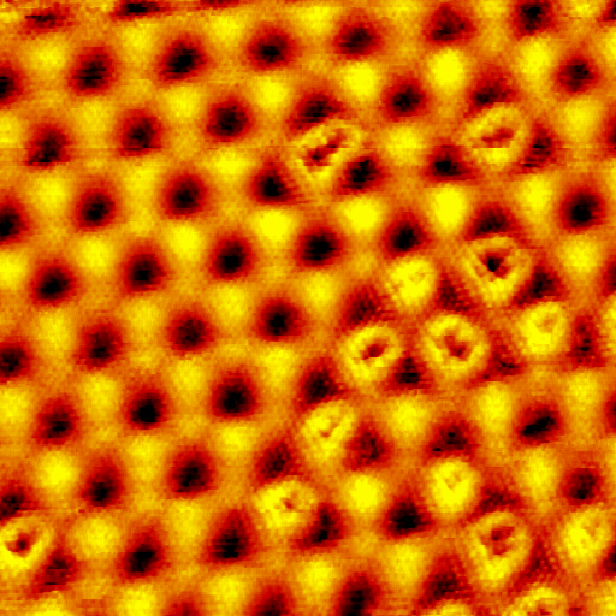
\includegraphics[height=\textwidth]{STMdata/FFT/2016-04-14_000_27.png}
    \caption{180x180Å - 1.020 nA 190.4 mV}
    \label{D2:15932}
  \end{subfigure}
  \begin{subfigure}[b]{0.3\paperwidth}
    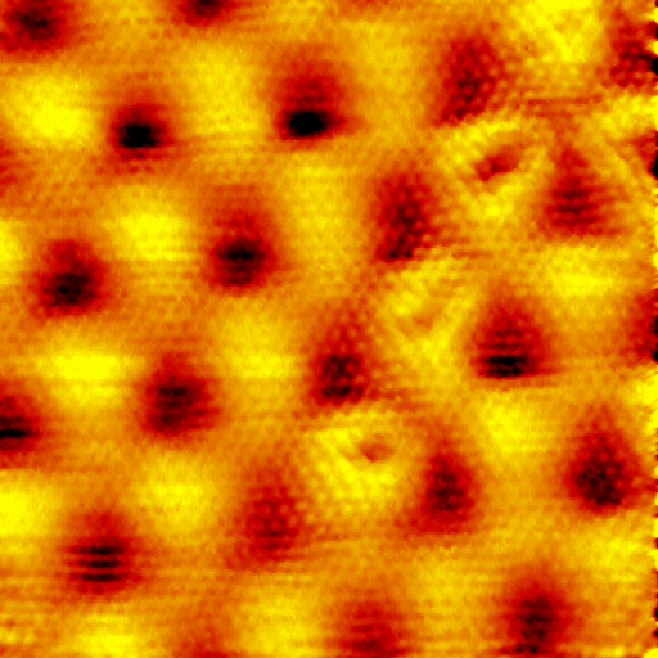
\includegraphics[height=\textwidth]{STMdata/FFT/2016-04-14_000_29.png}
    \caption{97x97 Å - 1.020 nA, 190.4 mV}
    \label{D2:15933}
  \end{subfigure}
}
\caption{Hydrogenated Gr/Ir surface after dose of H$_2$ at a doser temperature of 1593\degree C.}
\label{D2:1593}
\end{figure}

\subsection{1343\degree C dose}

The pirani pressure was measured to $6.8 \cdot 10^{-2}$mbar, and the doser had a temperature of 1343\degree C. Hydrogen was dosed for 20 min as earlier. As seen on figure \ref{D2:1340} several high quality pictures of the sample was taken. On figure \ref{D2:13401} it would seem like some hydrogen is adsorbed due to the several ring shaped structures. As a smaller image is taken such as the one in figure \ref{D2:13402} the defects looks somewhat different from those seen earlier on figures \ref{D2:15932} and \ref{D2:17453}. The ring shaped structures are much smaller in diameter on figure \ref{D2:13402}, even though the scanning parameters are close to each other.\\
A high resolution image is seen on figure \ref{D2:13403}, where the hexagonal graphene is highly visivble. On this picture it is clear that the graphene is defected, although it is unclear whether this is due to the presence of hydrogen. It is also seen that the shape of the sites in the moiré unit cell looks different than earlier although both pictures are from the same scan session. This is due to a tip effect, where the LDOS of the tip probably has changed, which has a influence on the tunneling current. This feature might happen if the tip picks up an atom from the surface, or if the physical dimensions of the tip changes after a tip treatment.\\
It should be noted that the graphene had defects before the dose was initiated. The abundance of these defects was indistinguishable, compared between before and after dosage. Therefore it is not possible to conclude whether the threshold temperature of the hydrogen adsorbtion from excited molecules lies at 1340\degree C. It is however very likely that no hydrogen is adsorbed. In order to investigate the threshold temperature further, it would be rational to conduct TPD measurements of the sample after hydrogen dosage at 1343 \degree C.

\begin{figure}[H]
\makebox[\textwidth][c]{
  \begin{subfigure}[b]{0.3\paperwidth}
    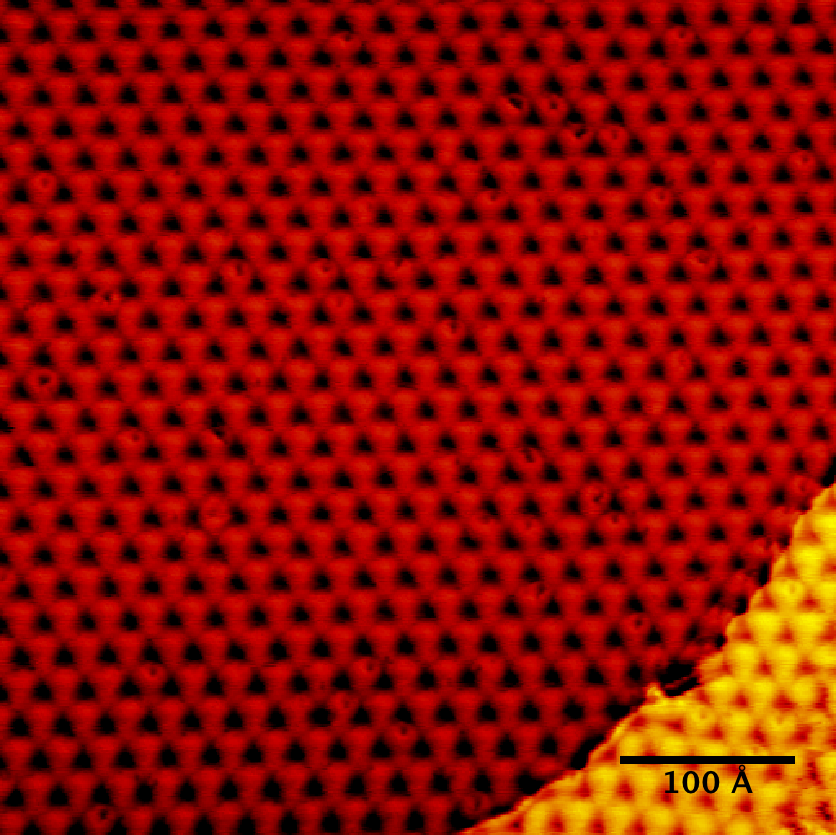
\includegraphics[height=\textwidth]{STMdata/FFT/2016-04-16_001_50_26.png}
    \caption{477x477 Å - 0.820 nA 20.1 mV}
    \label{D2:13401}
  \end{subfigure}
  \begin{subfigure}[b]{0.3\paperwidth}
    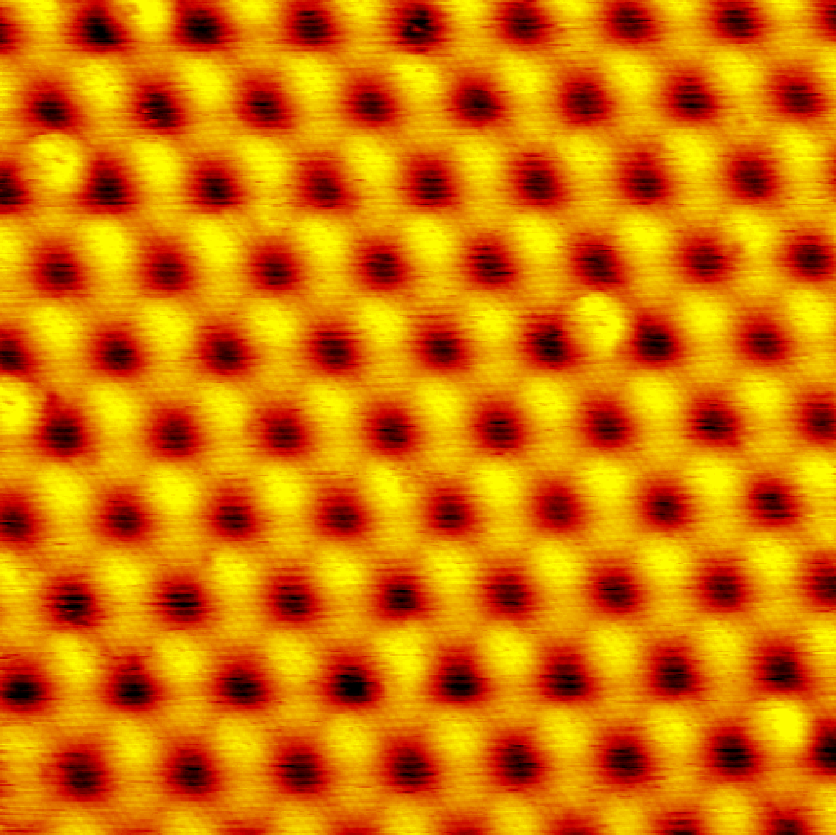
\includegraphics[height=\textwidth]{STMdata/FFT/2016-04-16_001_50_8.png}
    \caption{192x192Å - 0.830 nA 55.8 mV}
    \label{D2:13402}
  \end{subfigure}
  \begin{subfigure}[b]{0.3\paperwidth}
    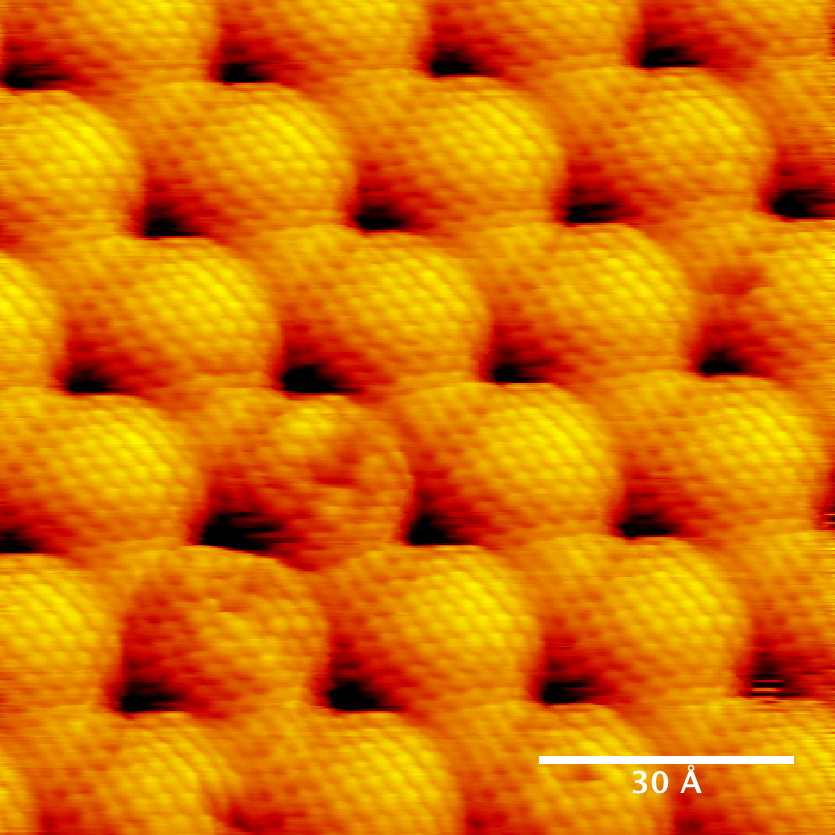
\includegraphics[height=\textwidth]{STMdata/FFT/2016-04-16_001_50_15.png}
    \caption{98x98 Å - 0.820 nA, 20.1 mV}
    \label{D2:13403}
  \end{subfigure}
}
\caption{Hydrogenated Gr/Ir surface after dose of H$_2$ at a doser temperature of 1340\degree C.}
\label{D2:1340}
\end{figure}



\section{TPD measurements - Atomic and molecular D2}

In figure \ref{TPD:all} below, the data from the TPD is gathered in two different figures. TPD measurements were made for both the vibrationally excited molecules and atoms. Figure \ref{TPD:D2} shows the data aquired for the D2 dose and figure \ref{TPD:D} shows the data for the dose with hot atoms. After dosage of excited molecules a single peak is observed. On figure \ref{TPD:D2} this peak is seen from two different datasets. It is worth noting that the peaks are shifted regarding to each other. The reasoin for this might be the fact that the sample was had different thermocouples, which has a big influence on the measured temperature. For the second dataset, corresponding to the blue graph, a quite big peak is seen after the main peak, at a temperature of about 800K. This is due to a temperature spike caused by the Eurotherm temperature controller. As shown in figure \ref{TPD:example} it is shown that a linear ramp of the temperature is desired. However the calibration of the Eurotherm during this experiment was poor, which results in noticeable fluctuations in the desorption of hydrogen. This implies that either the thermocouple adapts at a poor rate or that the desorption of hydrogen is sensitive to large changes in temperature. This phenomenon is also observed on figure \ref{TPD:D}, on the blue graph. This dataset was gathered during the same chamber and sample conditions as the blue graph in figure \ref{TPD:D2}. Therefore the calibration of the Eurotherm was poor as well, which is seen after the small peak at about 500K in figure \ref{TPD:D}. Here several small bumps are seen due to the non-constant change in temperature.\\
The temperature at the peak was found by the procedure described in chapter \ref{cha:procedure}. The single peak in figure \ref{TPD:D2} must correspond to the hydrogen adsorbed on the HCP and FCC sites in the moiré unit cell. This statement is supported by the preceding STM pictures that show no sign of hydrogen dimers in the ATOP sites. The temperature of this peak was found for 6 datasets in all, and the values of these are shown in the table below, along with the mean value.\\
\begin{table}
  \centering
  \makebox[\textwidth][c]{
  \begin{tabular}{c|c|c|c|c|c|c|c}
    Sample \# & Gr/Ir-\#1 & Gr/Ir-\#2 & Gr/Ir-\#3 & Gr/Ir-\#4 & Gr/Ir-\#5 & Gr/Ir-\#6 & mean \\
    \hline
    Peak T [K] & 724.8 & 698.4 & 694.0 & 709.1 & 739.1 & 753.4 & 719.8
  \end{tabular}}
\end{table}
Another peak appears when observing the Gr/Ir sample after it has been dosed with hot atoms as seen on figure \ref{TPD:D}. The green graph was initially observed, and from this it is obvious that more hydrogen desorps from the surface at lower temperature, compared to the green graph on figure \ref{TPD:D2}. After a second try however, an actual peak was observed. The temperature of this peak was found by the same procedures as earlier, and the value was found to be 550.4K. This suggests that a different type of Gr-H bond is present. The most plausible explanation is the presence of hydrogen dimers on the ATOP site of the moiré unit cell. The fact that no hydrogen adsorbs as dimers, when excited molecules are dosed, is supported heavily by the fact that this peak around 550K is completely absent from all the data obtained from the molecular dosage seen in figures \ref{TPD:D2} and \ref{TPD:bilayer}.

\begin{figure}
  \centering
  \begin{subfigure}[b]{0.45\textwidth}
    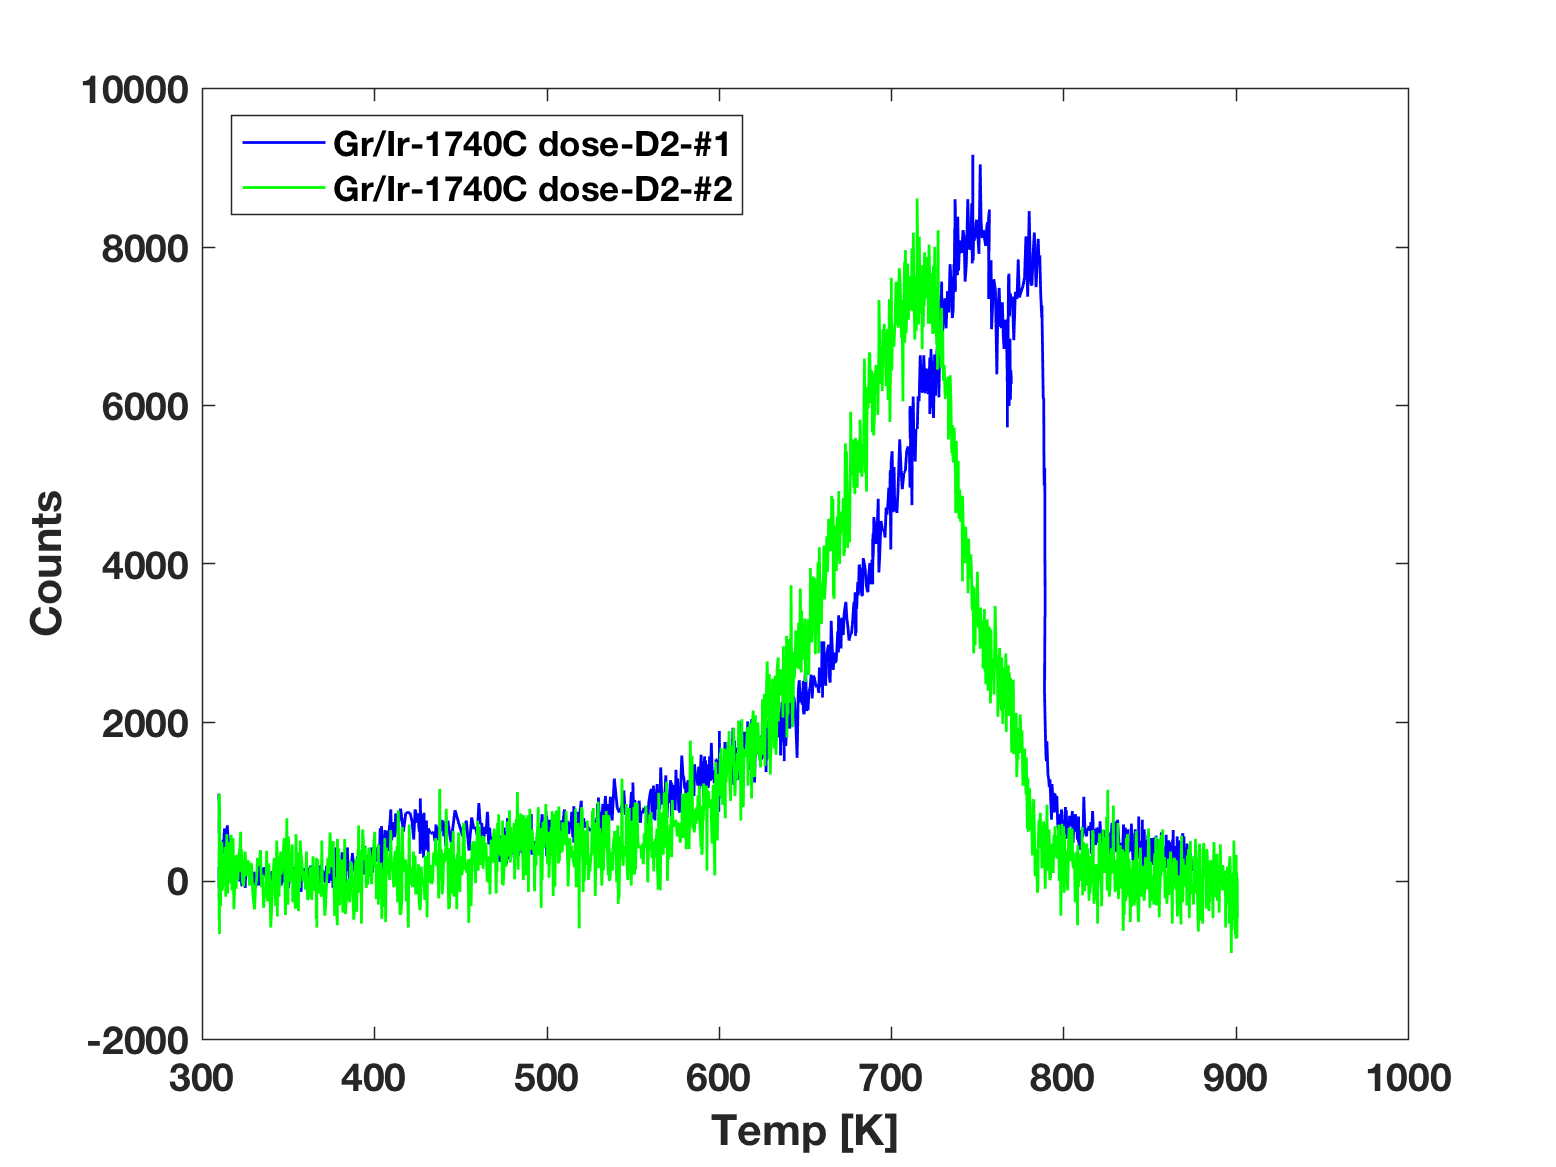
\includegraphics[width=\textwidth]{TPD/050516IrSorenD2dose1hourtemp.png}
    \caption{TPD of Gr/Ir after 1 hour dose of D$_2$ with a doser temperature of 1740 \degree C.}
    \label{TPD:D2}
  \end{subfigure}\hspace{0.5cm}
  \begin{subfigure}[b]{0.45\textwidth}
    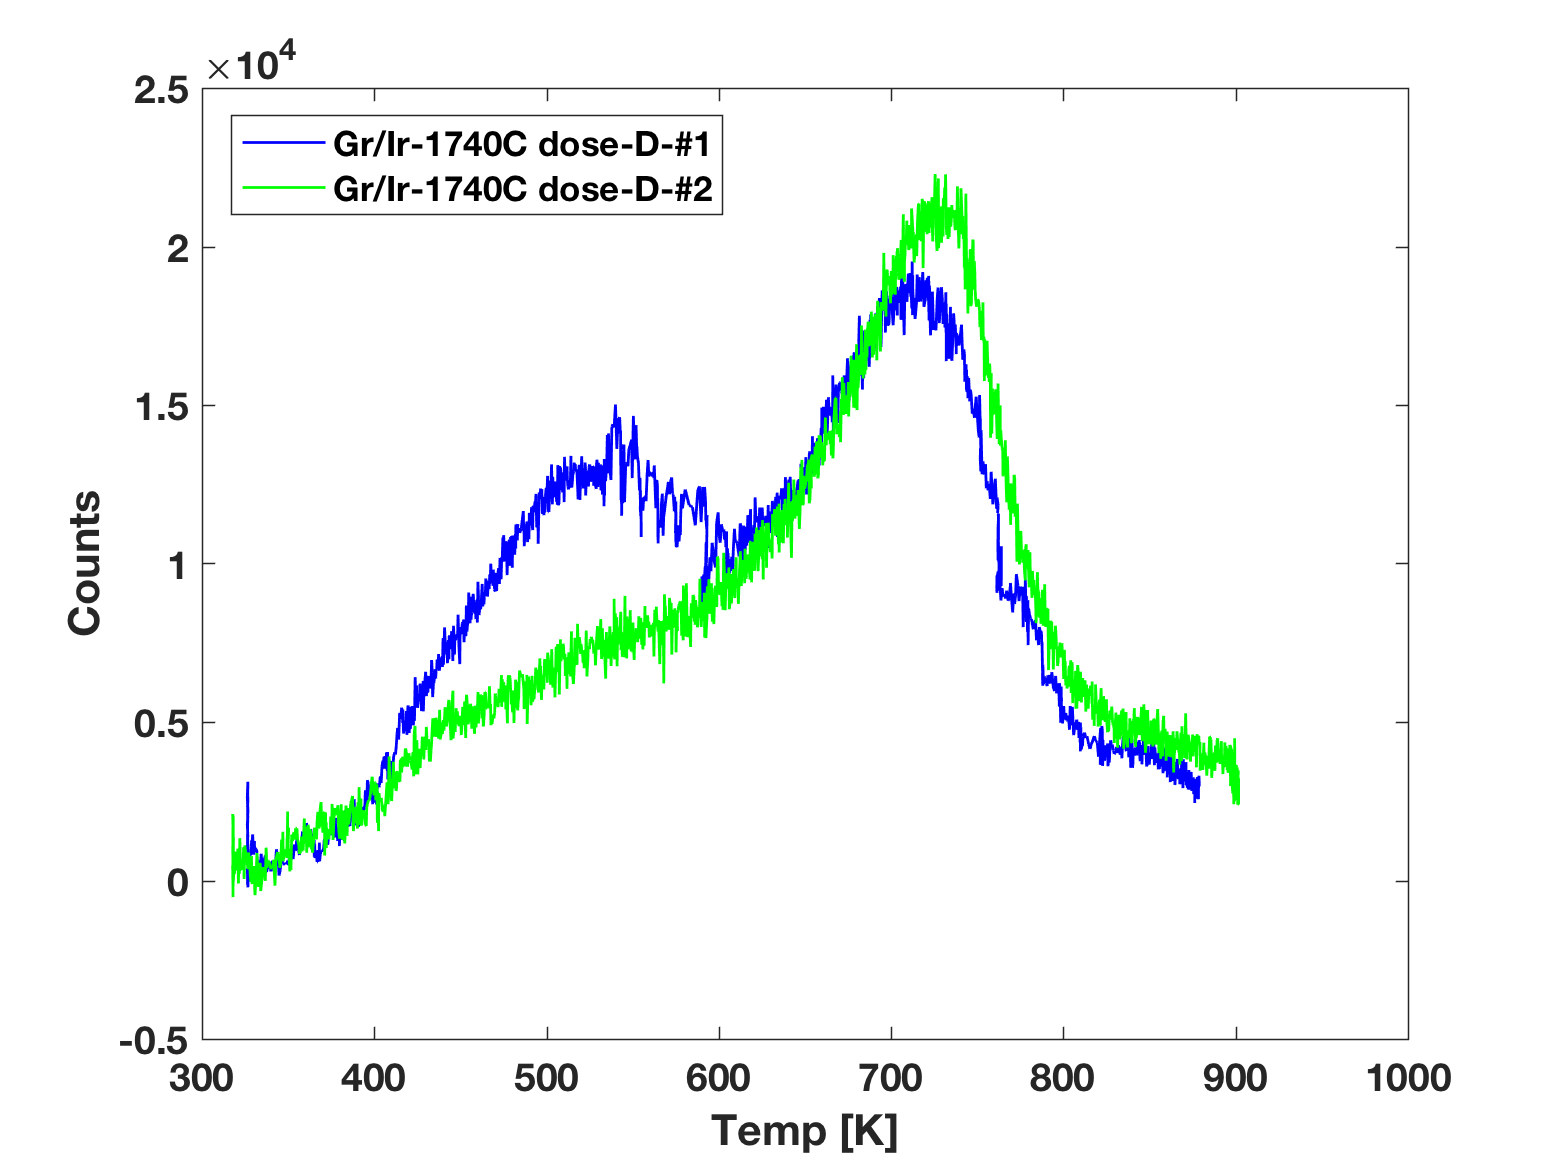
\includegraphics[width=\textwidth]{TPD/050516IrSorenDdose1hourtemp.png}
    \caption{TPD of Gr/Ir after 1 hour dose of atomic deuterium with a doser temperature of 1740 \degree C.}
    \label{TPD:D}
  \end{subfigure}
  \caption{}
  \label{TPD:all}
\end{figure}

As a further study of the adsorbtion of hydrogen on Gr/Ir, bilayers were grown on the sample by annealing in ethylene for a long period of time. STM pictures of these bilayers are shown in the following section. TPD measurements were however conducted on the sample before and after the long anneal. Vibrationally excited hydrogen molecules were dosed for an hour in order to saturate the surface. On figure \ref{TPD:bilayer} the red graph corresponds to the sample before the long anneal and the green graph corresponds to the sample after bilayers supposedly were grown. The background count of hydrogen was subtracted from both datasets and the same calibration is used to correct the temperature. It is seen that bilayers reduce the amount of hydrogen on the surface by a significant amount. This suggests that hydrogen is not adsorbed on the bilayered graphene. This theory is supported by the STM pictures below.\\
It should be noted that only two datasets were gathered from this experiment. The peak intensity from the TPD measurements tends to vary slightly and hence the amount of bilayers grown on the sample might not be perfectly related to the drop in peak intensity.


\begin{figure}[H]
  \centering
  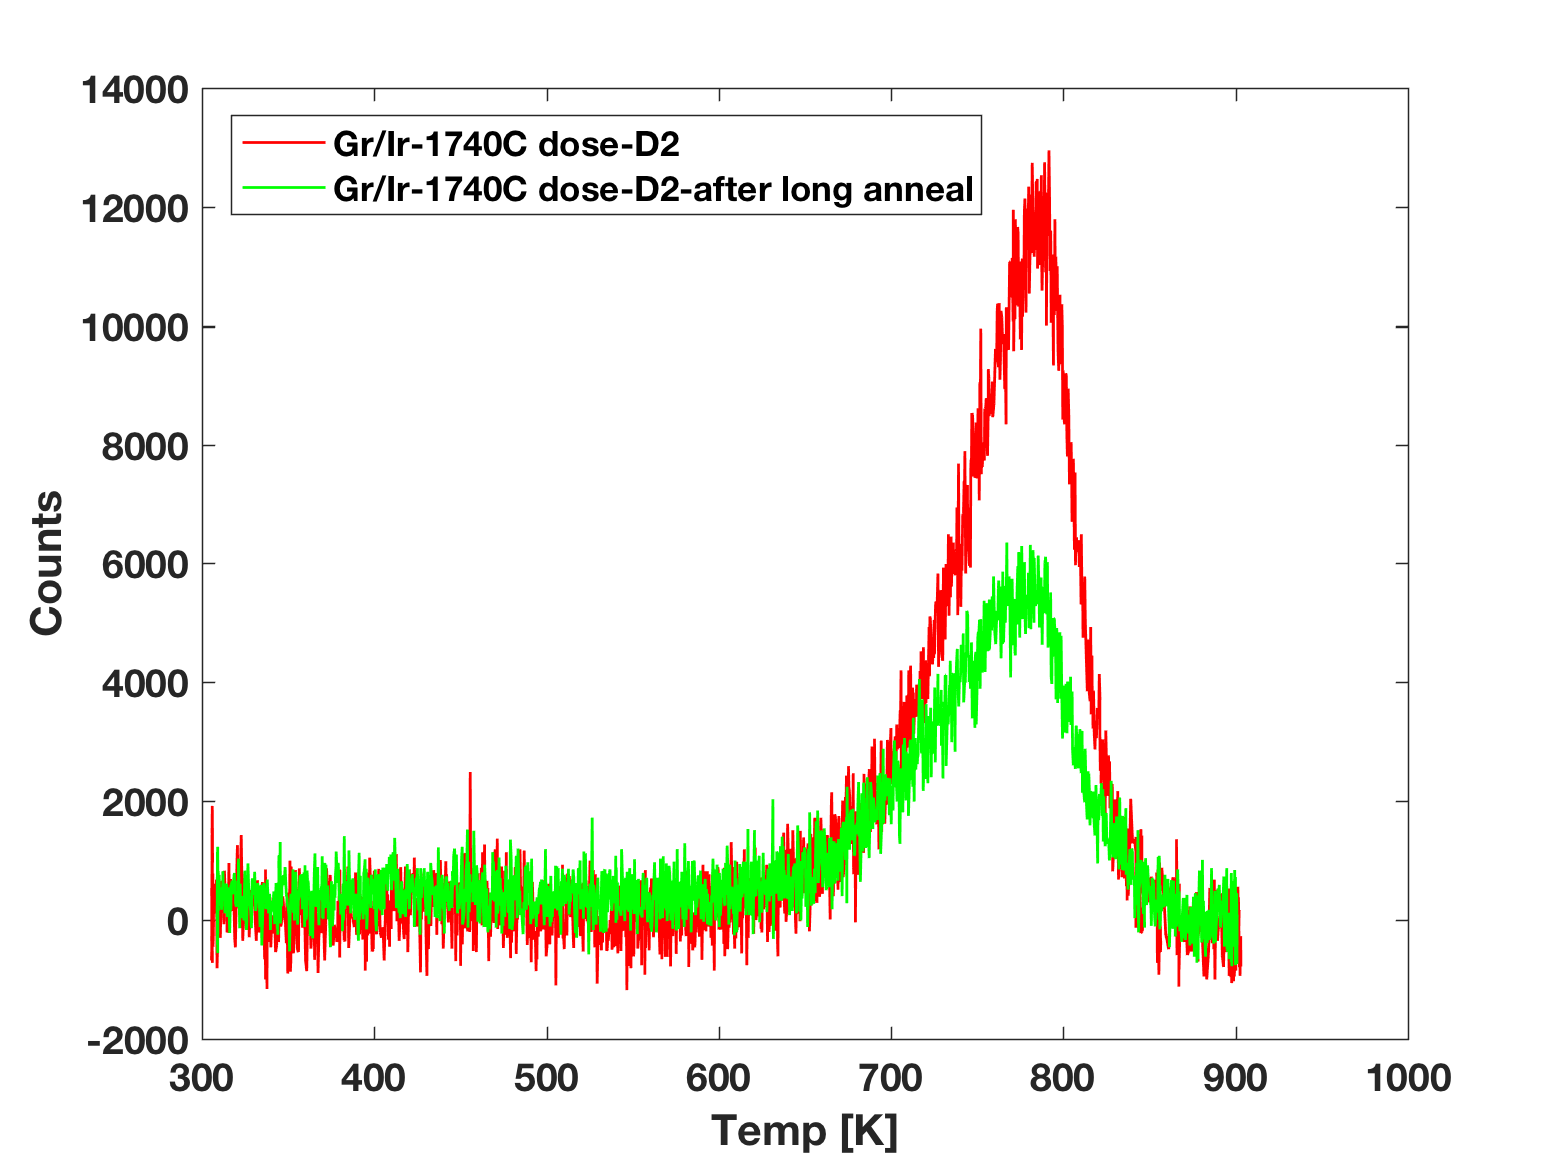
\includegraphics[width=0.6\textwidth]{TPD/GrIr1740CD2longannealtemp.png}
  \caption{}
  \label{TPD:bilayer}
\end{figure}

\section{Bilayered graphene on Ir}



\begin{figure}[H]
\makebox[\textwidth][c]{
  \begin{subfigure}[b]{0.3\paperwidth}
    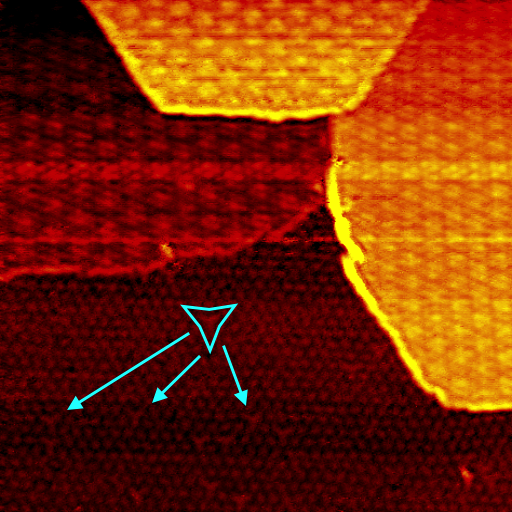
\includegraphics[height=\textwidth]{STMdata/FFT/2016-04-13_001_49.png}
    \caption{940x940 Å - 0.850 nA 75.7 mV}
    \label{D2:13401}
  \end{subfigure}
  \begin{subfigure}[b]{0.3\paperwidth}
    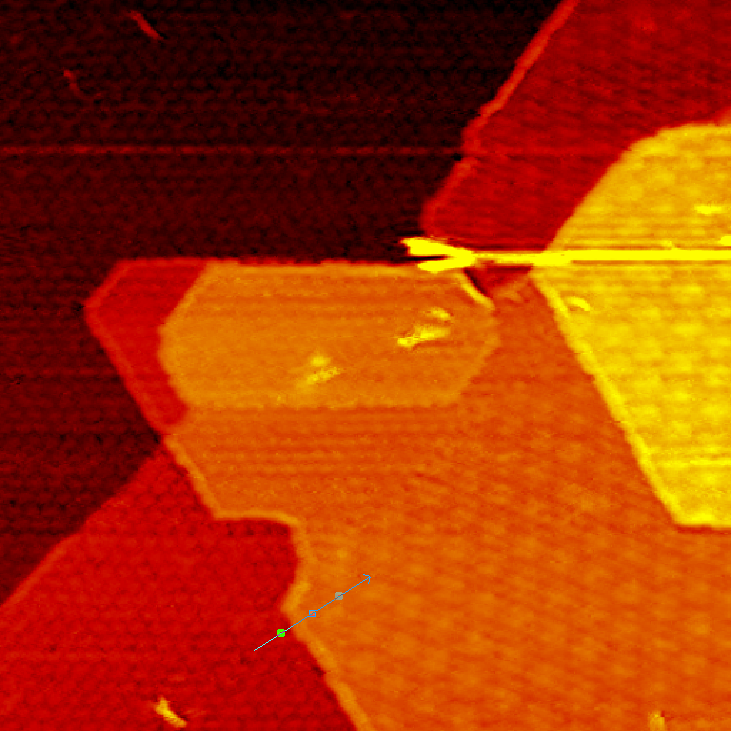
\includegraphics[height=\textwidth]{STMdata/FFT/2016-04-13_001_50.png}
    \caption{910x910Å - 0.800 nA 75.7 mV}
    \label{D2:13402}
  \end{subfigure}
  \begin{subfigure}[b]{0.3\paperwidth}
    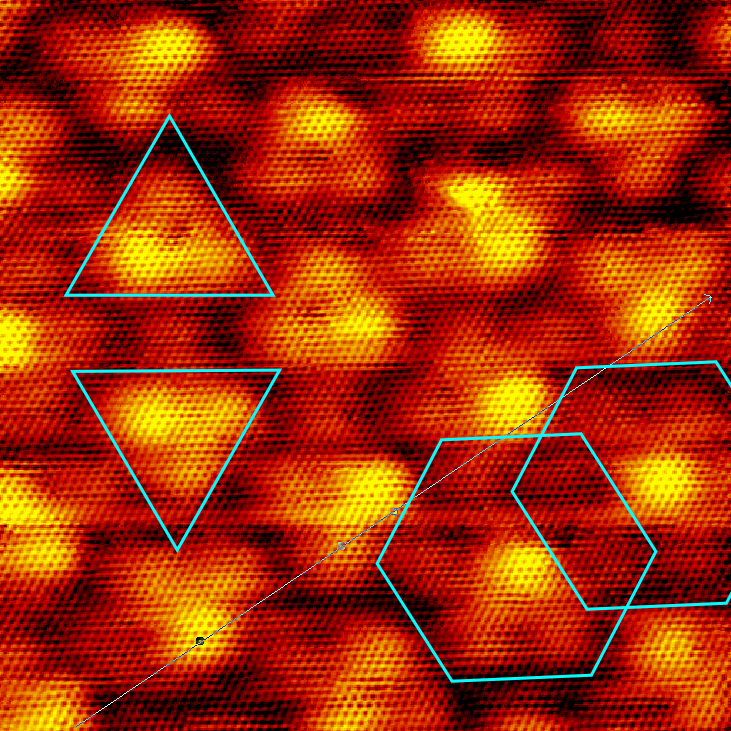
\includegraphics[height=\textwidth]{STMdata/FFT/2016-04-13_001_55.png}
    \caption{196x196 Å - 0.820 nA, 75.7 mV}
    \label{D2:13403}
  \end{subfigure}
}
\caption{Patches of bilayered graphene on Ir after a long hydrogen dosage.}
\label{D2:1340}
\end{figure}



\section{LEED of bilayered sample}

\begin{figure}[H]
\makebox[\textwidth][c]{
  \begin{subfigure}[b]{0.3\paperwidth}
    \includegraphics[height=\textwidth]{LEED/No" "flash/145eV.JPG}
    \caption{LEED without flashing. 145eV.}
    \label{}
  \end{subfigure}
  \begin{subfigure}[b]{0.3\paperwidth}
    \includegraphics[height=\textwidth]{LEED/Low" "T" "flash/145eV.JPG}
    \caption{LEED after low T flash. 145eV}
    \label{}
  \end{subfigure}
  \begin{subfigure}[b]{0.3\paperwidth}
    \includegraphics[height=\textwidth]{LEED/post" "1090" "flash/145eV.JPG}
    \caption{LEED after high T flash. 145eV}
    \label{}
  \end{subfigure}
}
\caption{}
\label{}
\end{figure}
